\documentclass[aspectratio=169]{beamer}

\usetheme{Madrid}
\usecolortheme{DSLAB}
\usefonttheme[onlylarge]{structurebold}
\setbeamerfont*{frametitle}{size=\normalsize,series=\bfseries}
\setbeamertemplate{navigation symbols}{}

\usepackage[utf8]{inputenc} 
\usepackage[T1]{fontenc}
\usepackage[english]{babel}
\usepackage{xmpmulti}
\usepackage{tikz}
\usepackage{pgf}
\usepackage{amsmath}
\usepackage{amsfonts}
\usepackage{graphicx}
\usepackage{color}
\usepackage{multirow}
\usepackage{lmodern}
\usepackage{hyperref}
\usepackage{eurosym}
\usepackage{listings}
\usepackage{booktabs}

\lstset{
  basicstyle=\ttfamily\small,
  frame=single,
  breaklines=true,
  showstringspaces=false,
  columns=fullflexible
}


\usetikzlibrary{arrows}
\tikzstyle{block}=[draw opacity=0.7,line width=1.4cm]

\setbeamercovered{dynamic}
\setbeamerfont{author}{family=\rmfamily}
\institute[URJC]{DSLAB}

\author[Big Data Processing II]{
	Alberto Fernández Isabel \\
	Natalia Madrueño Sierro \\
	Rubén Rodríguez Fernández \\
}

\title[Presentación]{
	Big Data Processing II \\ \vspace{0.2em}
	IA Generativa aplicada al deporte \\ \vspace{0.2em}
    Sistemas basados en agentes
}
\date{Marzo 2026}
\titlegraphic{
\includegraphics[width=3cm]{images/logos/logourjceps.png}}


\setbeamertemplate{section page}{
	\vspace{1cm}
	\begin{beamercolorbox}[sep=8pt,center,wd=\textwidth]{section title}
		\usebeamerfont{section title}\insertsection\par 
	\end{beamercolorbox}
}

\begin{document}

\begin{frame}
\titlepage
\end{frame}

%------------------------------------------------
\section{Mapa del bloque}
\frame{\sectionpage}

\begin{frame}{Arquitectura conceptual del bloque}
\begin{center}
\Large
\begin{tabular}{c}
{\color{gray2}\textbf{Sesión 1}} \\ 
{\color{gray2}Control del comportamiento} \\
{\color{gray2}\small Prompt Engineering + Post-training}
\\[0.1em]
$\Downarrow$
\\[0.1em]
{\color{gray2}\textbf{Sesión 2}} \\ 
{\color{gray2}Control de la información} \\
{\color{gray2}\small Retrieval-Augmented Generation (RAG)}
\\[0.1em]
$\Downarrow$
\\[0.1em]
{\color{colorblue}\textbf{Sesión 3}} \\ 
{\color{colorblue}Control del flujo y la acción} \\
{\color{colorblue}\small Agentes, Tools y Arquitecturas Cognitivas}
\end{tabular}
\end{center}
\end{frame}


\section{Introducción}
\frame{\sectionpage}

\begin{frame}{Del LLM reactivo al agente cognitivo}
\begin{columns}[T]
\column{0.5\textwidth}
Un LLM tradicional:

\[
Output = f(prompt)
\]

Un agente:

\[
acción_{t+1} = f(estado_t, objetivo, observación_t)
\]

\begin{itemize}
\item No solo responde.
\item Decide.
\item Actúa.
\item Aprende del entorno.
\end{itemize}

\column{0.5\textwidth}
\vspace{2em}
\centering
 
\includegraphics[width=0.9\textwidth]{images/presentacion/agents.png}
\end{columns}

\end{frame}

%------------------------------------------------
\begin{frame}{Por qué necesitamos agentes}
\begin{columns}[T]
\column{0.5\textwidth}
LLM + RAG permiten:

\begin{itemize}
\item Responder preguntas.
\item Sintetizar información.
\end{itemize}

Pero no permiten:

\begin{itemize}
\item Ejecutar \textbf{cálculos complejos}.
\item \textbf{Consultar} múltiples sistemas.
\item \textbf{Tomar decisiones} secuenciales.
\item \textbf{Adaptarse dinámicamente}.
\end{itemize}

\column{0.5\textwidth}
\vspace{2em}
\centering
 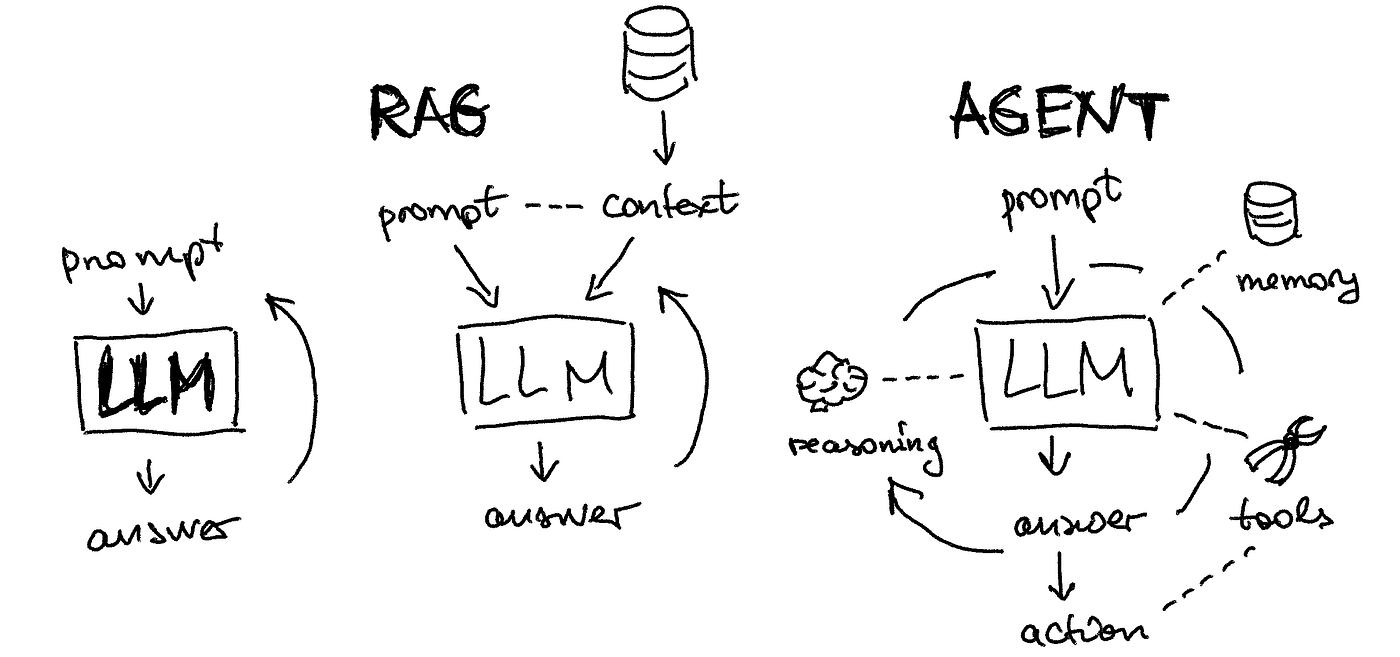
\includegraphics[width=0.9\textwidth]{images/presentacion/ragagents.png}
\end{columns}

\end{frame}

%------------------------------------------------
\section{Skills y tools}
\frame{\sectionpage}

\begin{frame}{Skills: capacidades operativas}
\begin{columns}[T]
\column{0.5\textwidth}
Un agente se compone de \textbf{habilidades (skills)}:
\begin{itemize}
\item consultar bases de datos
\item ejecutar modelos estadísticos
\item calcular métricas avanzadas
\item generar visualizaciones
\item enviar alertas automáticas
\end{itemize}
Un skill es una \textbf{capacidad reutilizable}.

\column{0.5\textwidth}
\vspace{2em}
\centering
 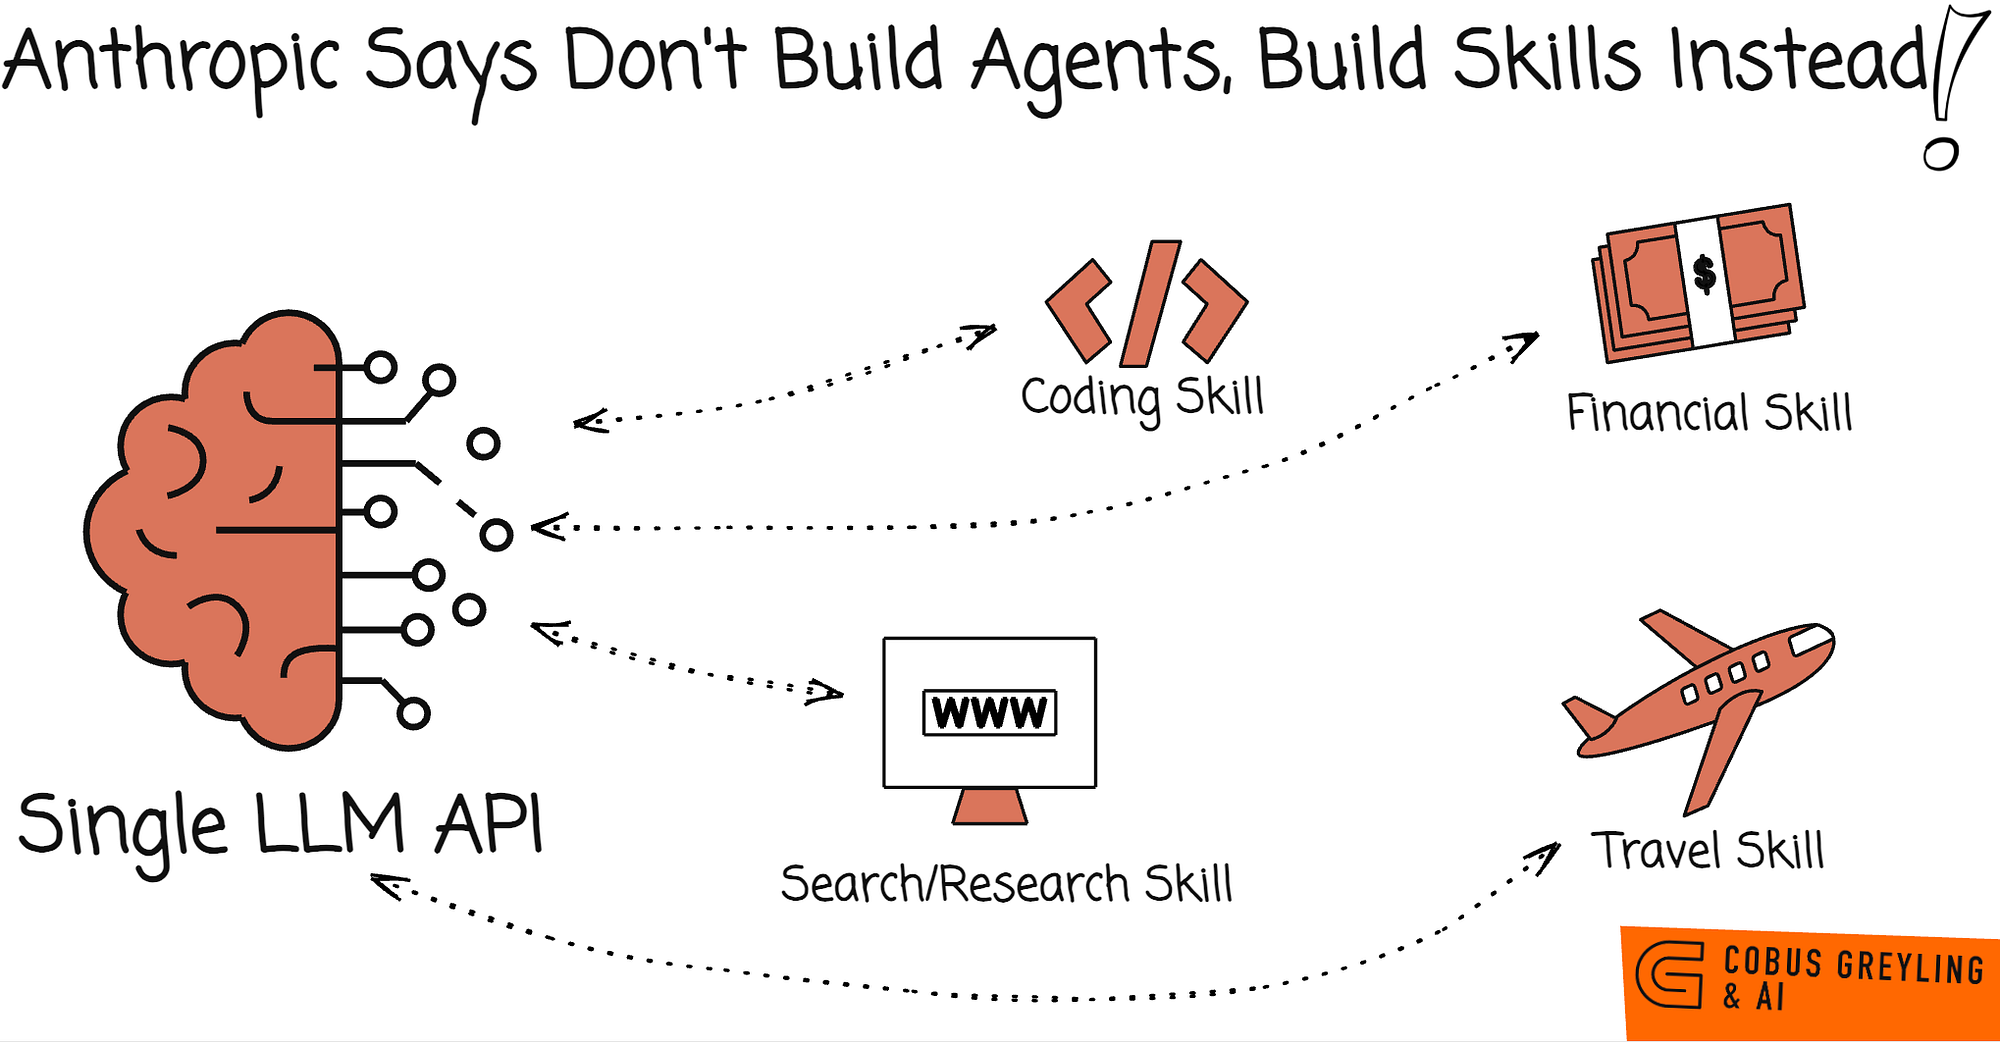
\includegraphics[width=0.9\textwidth]{images/presentacion/skills.png}
\end{columns}
\end{frame}

%------------------------------------------------
\begin{frame}{Tools vs Skills}
\centering
\begin{tabular}{ll}
\toprule
\textbf{Tool} & \textbf{Skill} \\
\midrule
Función aislada & Capacidad compuesta \\
Ejecuta acción & Orquesta acciones \\
Ej: query DB & Ej: análisis rendimiento \\
\bottomrule
\end{tabular}
\end{frame}

%------------------------------------------------
\begin{frame}{Ecosistema de herramientas}
\begin{columns}[T]
\column{0.5\textwidth}
Ejemplos en deporte:

\begin{itemize}
\item API de tracking físico.
\item Motor de cálculo de xG (goles esperados).
\item Base histórica de rendimiento.
\item Generador de dashboards.
\end{itemize}

El valor del agente crece con su ecosistema.

\column{0.5\textwidth}
\centering
 
\includegraphics[width=0.9\textwidth]{images/presentacion/agentsai.jpg}
\end{columns}
\end{frame}

%------------------------------------------------
\section{Planificación y razonamiento iterativo}
\frame{\sectionpage}

\begin{frame}{Razonamiento iterativo}
\begin{columns}[T]
\column{0.5\textwidth}
Los agentes complejos no actúan en un solo paso. \\
\vspace{1em}
Proceso:

\begin{enumerate}
\item\textbf{Analizar objetivo}.
\item \textbf{Descomponer subtareas}.
\item \textbf{Ejecutar pasos}.
\item \textbf{Evaluar resultados}.
\item \textbf{Continuar o finalizar}.
\end{enumerate}

\column{0.5\textwidth}
\centering
 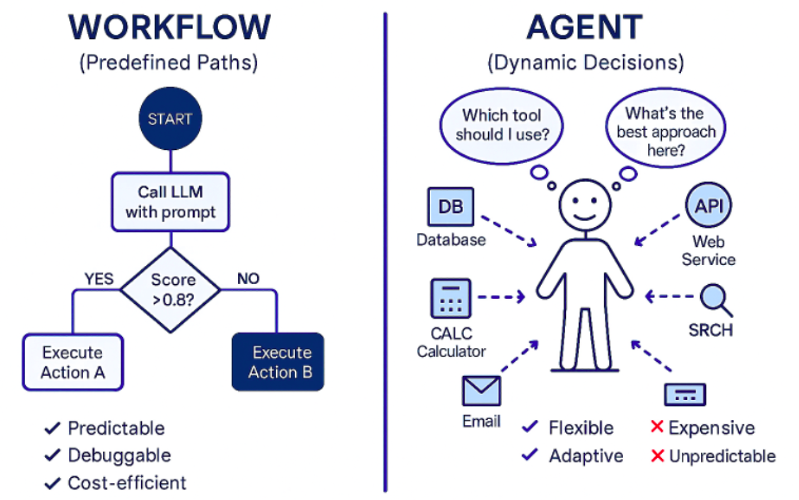
\includegraphics[width=0.9\textwidth]{images/presentacion/agentsflow.png}
\end{columns}

\end{frame}

%------------------------------------------------
\begin{frame}{ReAct: Reasoning + Acting}
\begin{columns}[T]
\column{0.5\textwidth}
Arquitectura \textbf{ReAct}:

\begin{itemize}
\item \textbf{Pensamiento} intermedio.
\item \textbf{Selección} de acción.
\item \textbf{Ejecución} de tool.
\item \textbf{Observación} del resultado.
\item \textbf{Iteración}.
\end{itemize}

Combina \textbf{razonamiento y acción}.
\column{0.5\textwidth}
\centering
 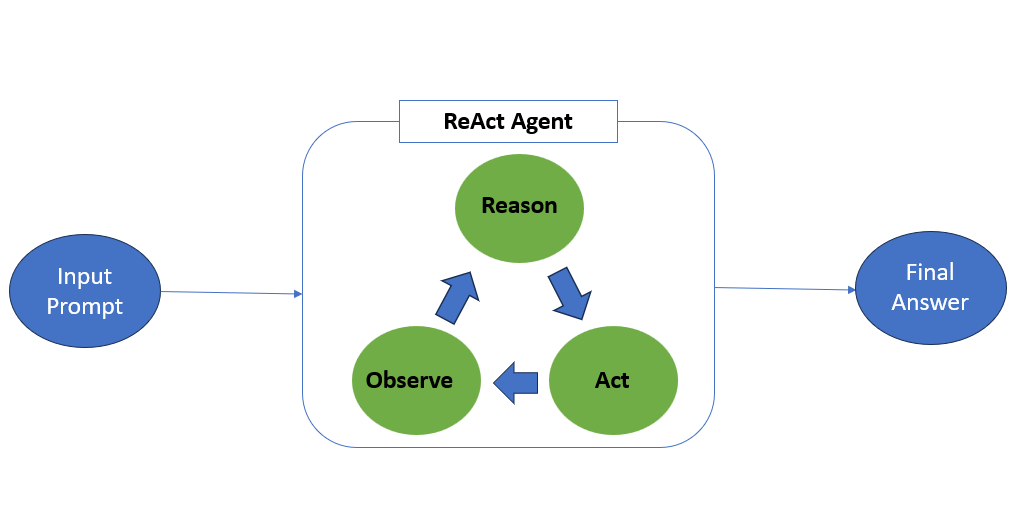
\includegraphics[width=0.98\textwidth]{images/presentacion/react.png}
\end{columns}
\end{frame}

%------------------------------------------------
\begin{frame}{Planner-Executor}
\begin{columns}[T]
\column{0.5\textwidth}
Arquitectura \textbf{moderna}:

\begin{itemize}
\item \textbf{Planner}: diseña los pasos
\item \textbf{Executor}: ejecuta herramientas
\item \textbf{Evaluator}: valida resultados
\end{itemize}

Permite tareas complejas multi-etapa.
\column{0.5\textwidth}
\centering
 
\includegraphics[width=0.98\textwidth]{images/presentacion/orchestrator.jpg}
\end{columns}
\end{frame}

%------------------------------------------------
\section{Arquitecturas dirigidas por estado (control de flujo)}
\frame{\sectionpage}
\begin{frame}{Por qué no basta con chains lineales}
Los flujos lineales (chains) fallan cuando:
\begin{itemize}
    \item La ruta depende del contenido (distintos casos de uso).
    \item Hay pasos opcionales (solo si faltan datos, solo si hay anomalía).
    \item Hay iteración (refinar consulta, reintentar retrieval, validar).
    \item Se necesitan \textbf{invariantes} (no continuar si el JSON no valida).
\end{itemize}

\vspace{0.3em}
\textbf{Necesidad:} control explícito del flujo y de las condiciones de parada.
\end{frame}

\begin{frame}{Agentes como máquinas de estados}
\begin{columns}[T]
\column{0.5\textwidth}
Una forma rigurosa de diseñar agentes es modelarlos como:
\[
S \xrightarrow{evento/condición} S'
\]

\begin{itemize}
    \item \textbf{Estados} = etapas del proceso (retrieve, compute, write-report, validate).
    \item \textbf{Transiciones} = reglas (si falta dato → consultar DB; si inconsistente → reintentar).
    \item \textbf{Guardas} = condiciones que evitan errores (no generar si no hay evidencias).
\end{itemize}

\vspace{0.3em}
\textbf{Ventaja:} control del sistema > “improvisación del LLM”.

\column{0.5\textwidth}
\vspace{1em}
\centering
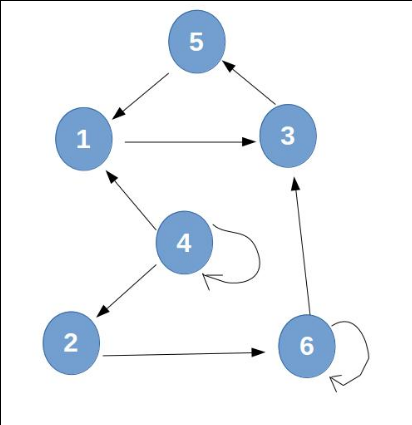
\includegraphics[width=0.7\textwidth]{images/presentacion/states.png}
\end{columns}
\end{frame}

\begin{frame}{Patrones de control de flujo útiles}
\begin{columns}[T]
\column{0.5\textwidth}
Patrones típicos en agentes:
\begin{itemize}
    \item \textbf{Router}: elegir herramienta según intención (consulta histórica vs cálculo).
    \item \textbf{Validator}: comprobar esquema/consistencia antes de seguir.
    \item \textbf{Retry with backoff}: reintentos controlados ante fallos de tool/timeout.
    \item \textbf{Loop bounded}: iteración con límite de pasos para evitar loops infinitos.
\end{itemize}

\vspace{0.3em}
\textbf{Idea clave:} la robustez viene del control de flujo, no del “prompt perfecto”.
\column{0.5\textwidth}
\vspace{1em}
\centering
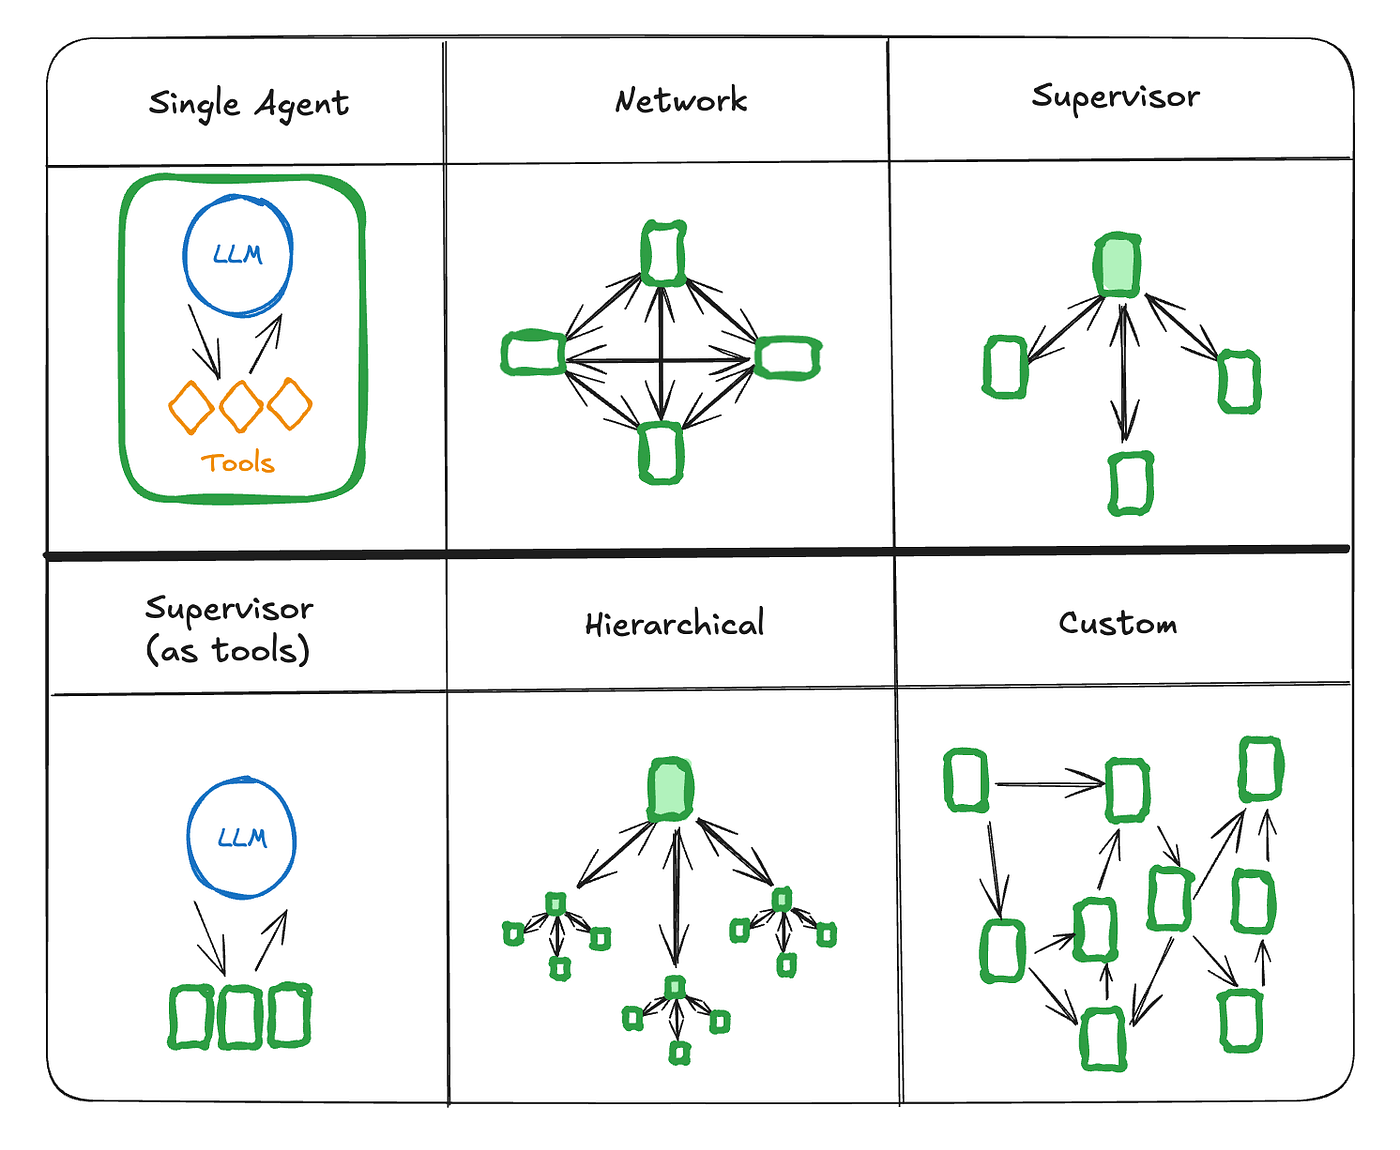
\includegraphics[width=0.9\textwidth]{images/presentacion/patterns.png}
\end{columns}
\end{frame}

\begin{frame}{Ejemplo deportivo: agente de informe post-partido}
\textbf{Estados de alto nivel:} \\
\centering
\begin{tikzpicture}[
    node distance=1.3cm,
    every node/.style={font=\small},
    process/.style={
        rectangle,
        rounded corners,
        draw=colorblue,
        fill=colorblue!15,
        align=center,
        minimum width=6.8cm,
        minimum height=1.0cm,
        line width=1pt
    },
    arrow/.style={->, thick, draw=colorblue}
]

\node (fetch) [process]
{\textbf{Fetch}\\ \footnotesize recuperar datos del partido (eventos + tracking)};

\node (compute) [process, below of=fetch]
{\textbf{Compute}\\ \footnotesize calcular métricas derivadas (xG, PPDA, cargas)};

\node (compare) [process, below of=compute]
{\textbf{Compare}\\ \footnotesize contrastar con histórico (últimos $N$ partidos)};

\node (draft) [process, below of=compare]
{\textbf{Draft}\\ \footnotesize generar informe estructurado};

\node (validate) [process, below of=draft]
{\textbf{Validate}\\ \footnotesize validar esquema + coherencia con evidencias};

\draw [arrow] (fetch) -- (compute);
\draw [arrow] (compute) -- (compare);
\draw [arrow] (compare) -- (draft);
\draw [arrow] (draft) -- (validate);

\end{tikzpicture}


\vspace{0.3em}
\textbf{Routing:} si faltan métricas → volver a Fetch; si el JSON falla → volver a Draft.
\end{frame}

\begin{frame}{Riesgos y mitigación en control de flujo}
\begin{itemize}
    \item \textbf{Loops infinitos}: imponer límite de iteraciones y condiciones de parada.
    \item \textbf{Tool misuse}: validación de argumentos + esquemas estrictos.
    \item \textbf{Saltos incorrectos}: transiciones solo si se cumplen guardas.
    \item \textbf{Acumulación de latencia}: cortar ramas no necesarias y cachear resultados.
\end{itemize}

\vspace{0.3em}
\textbf{Conclusión:} el estado gobierna el flujo; el LLM decide dentro de límites.
\end{frame}


%------------------------------------------------
\section{Memoria y estado}
\frame{\sectionpage}
%------------------------------------------------
\section{Memoria (persistencia) y estado (representación)}

\begin{frame}{Diferencia crítica: estado vs memoria}
\textbf{Estado}:
\begin{itemize}
    \item Representación del \textbf{proceso actual} (qué sabemos ahora y qué falta).
    \item Vive dentro de la ejecución (por ejemplo, un diccionario/JSON de trabajo).
\end{itemize}

\vspace{0.4em}
\textbf{Memoria}:
\begin{itemize}
    \item Persistencia entre ejecuciones: historial, preferencias, perfiles, conocimiento externo.
    \item Vive fuera del flujo principal (DB, vector store, logs, cache).
\end{itemize}

\vspace{0.3em}
\textbf{Problema habitual:} mezclar ambos genera agentes incoherentes y difíciles de depurar.
\end{frame}

\begin{frame}{Memoria: cuatro tipos prácticos}
\begin{columns}[T]
\column{0.5\textwidth}
\begin{itemize}
    \item \textbf{Conversacional (corto plazo)}: historial reciente (context window).
    \item \textbf{Episódica}: interacciones previas resumidas (resúmenes por sesión).
    \item \textbf{Semántica}: documentos y conocimiento recuperable (RAG).
    \item \textbf{Estructurada}: perfiles, preferencias, configuraciones (tablas/JSON persistente).
\end{itemize}

\vspace{0.3em}
\textbf{Idea clave:} cada tipo tiene coste, latencia y riesgos distintos.

\column{0.5\textwidth}
\vspace{1em}
\centering
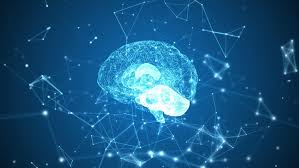
\includegraphics[width=0.9\textwidth]{images/presentacion/brain.jpg}
\end{columns}
\end{frame}

\begin{frame}{Diseño de memoria: decisiones de ingeniería}
\begin{columns}[T]
\column{0.5\textwidth}
Preguntas que deben tener respuesta:
\begin{itemize}
    \item \textbf{Qué se guarda} (señal vs ruido).
    \item \textbf{Cuándo se guarda} (al final de tarea, tras validación).
    \item \textbf{Cómo se recupera} (por claves, por embeddings, por filtros).
    \item \textbf{Caducidad} (TTL): lo viejo puede perjudicar.
    \item \textbf{Auditoría}: logs trazables para explicar decisiones.
\end{itemize}

\vspace{0.3em}
\textbf{Objetivo:} memoria útil, no acumulación de texto.

\column{0.5\textwidth}
\vspace{1em}
\centering

\includegraphics[width=0.9\textwidth]{images/presentacion/aibrain.jpg}
\end{columns}
\end{frame}

\begin{frame}{Ejemplo deportivo: memoria en un agente de scouting}
\textbf{Memoria estructurada:} perfil del jugador (posición, rol, minutos, lesiones). \\
\textbf{Memoria semántica:} informes textuales de scouting y clips anotados. \\
\textbf{Memoria episódica:} decisiones previas del agente (por qué recomendó A vs B).

\vspace{0.4em}
Consulta:
\begin{quote}
“Dame 3 perfiles similares a este extremo, justificando con evidencias de informes.”
\end{quote}

\textbf{Resultado:} respuestas consistentes porque el agente recuerda y cita.
\end{frame}

\begin{frame}{Riesgos típicos de memoria y cómo mitigarlos}
\begin{columns}[T]
\column{0.5\textwidth}
\begin{itemize}
    \item \textbf{Contaminación} (guardar alucinaciones) → guardar solo tras validación.
    \item \textbf{Obsolescencia} → TTL y versionado (temporada, fecha, fuente).
    \item \textbf{Privacidad/seguridad} → control de acceso + minimización de datos.
    \item \textbf{Sesgo por historiales} → resumir y normalizar, no copiar todo.
\end{itemize}

\vspace{0.3em}
\textbf{Conclusión:} la memoria aumenta capacidad, pero sin control degrada fiabilidad.
\column{0.5\textwidth}
\vspace{3em}
\centering
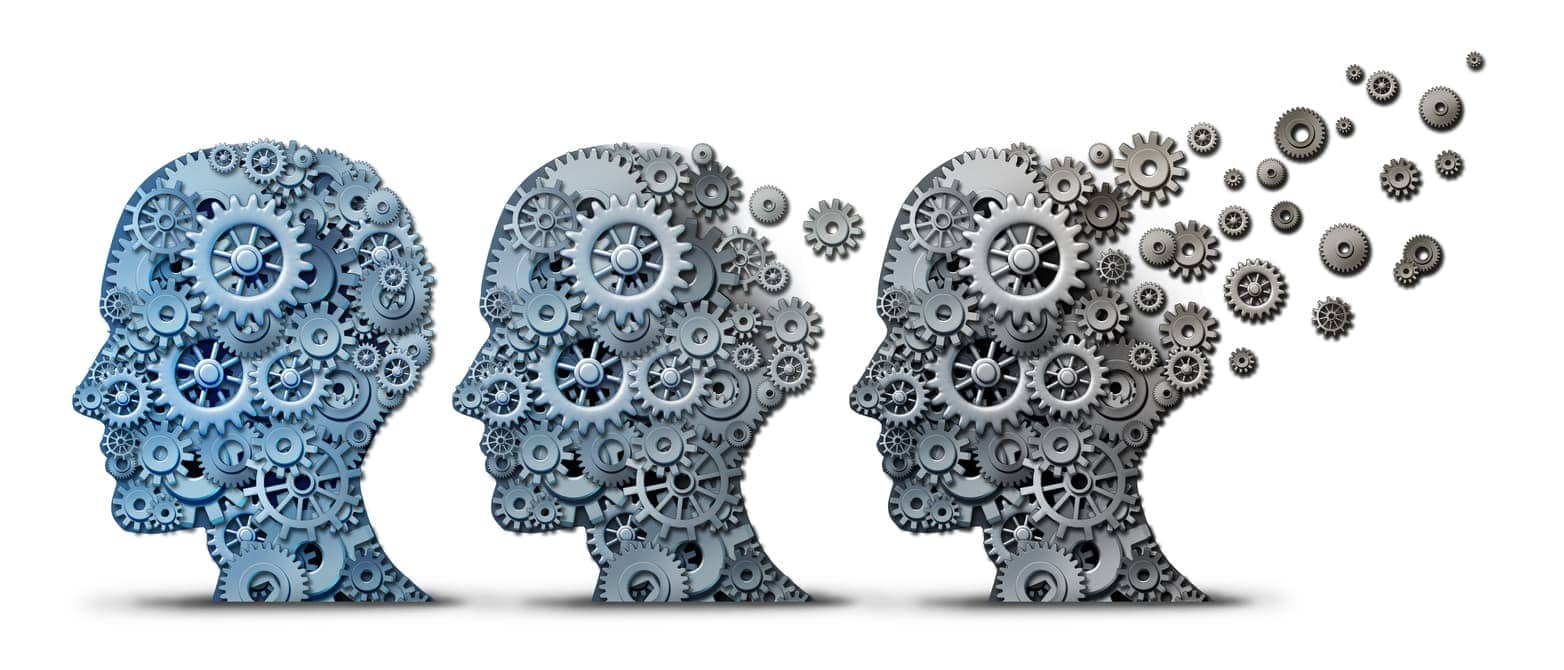
\includegraphics[width=0.9\textwidth]{images/presentacion/memoryrisk.jpg}
\end{columns}
\end{frame}

%------------------------------------------------
\section{Riesgos y fallos reales en agentes}
\frame{\sectionpage}

\begin{frame}{Complejidad sistémica}
\begin{columns}[T]
\column{0.5\textwidth}
A mayor autonomía del agente:

\begin{itemize}
    \item mayor número de componentes,
    \item mayor superficie de fallo,
    \item mayor dificultad de depuración.
\end{itemize}

Los fallos rara vez provienen del modelo aislado. \\
\vspace{1em}
\textbf{Conclusión:} la memoria aumenta capacidad, pero sin control degrada fiabilidad.
\column{0.5\textwidth}
\centering
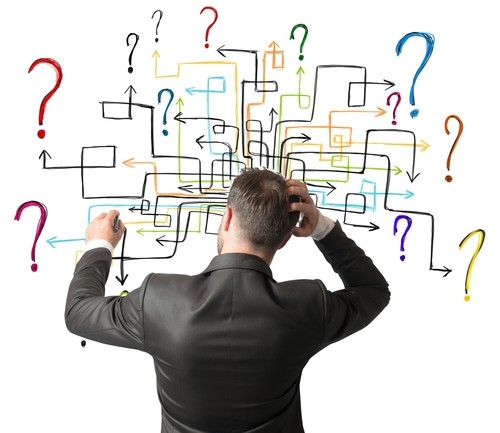
\includegraphics[width=0.9\textwidth]{images/presentacion/complex.jpg}
\end{columns}
\end{frame}

%------------------------------------------------

\begin{frame}{Loops y planificación incorrecta}
\begin{columns}[T]
\column{0.5\textwidth}
\textbf{Problemas frecuentes:}
\begin{itemize}
    \item iteraciones sin condición de parada,
    \item reintentos infinitos de retrieval,
    \item planificación redundante.
\end{itemize}
\vspace{1em}
\textbf{Mitigación:}
\begin{itemize}
    \item límites de iteración,
    \item condiciones de parada explícitas,
    \item control del estado.
\end{itemize}
\vspace{1em}
\textbf{Conclusión:} la memoria aumenta capacidad, pero sin control degrada fiabilidad.
\column{0.5\textwidth}
\vspace{3em}
\centering

\includegraphics[width=0.6\textwidth]{images/presentacion/loop.png}
\end{columns}
\end{frame}

%------------------------------------------------

\begin{frame}{Uso incorrecto de herramientas}
\begin{columns}[T]
\column{0.5\textwidth}
\textbf{El agente puede:}

\begin{itemize}
    \item invocar tools equivocadas,
    \item usar parámetros inválidos,
    \item interpretar mal los resultados.
\end{itemize}
\vspace{1em}
\textbf{Mitigación:}

\begin{itemize}
    \item esquemas de entrada estrictos,
    \item validación automática,
    \item manejo robusto de errores.
\end{itemize}

\column{0.5\textwidth}
\vspace{1em}
\centering
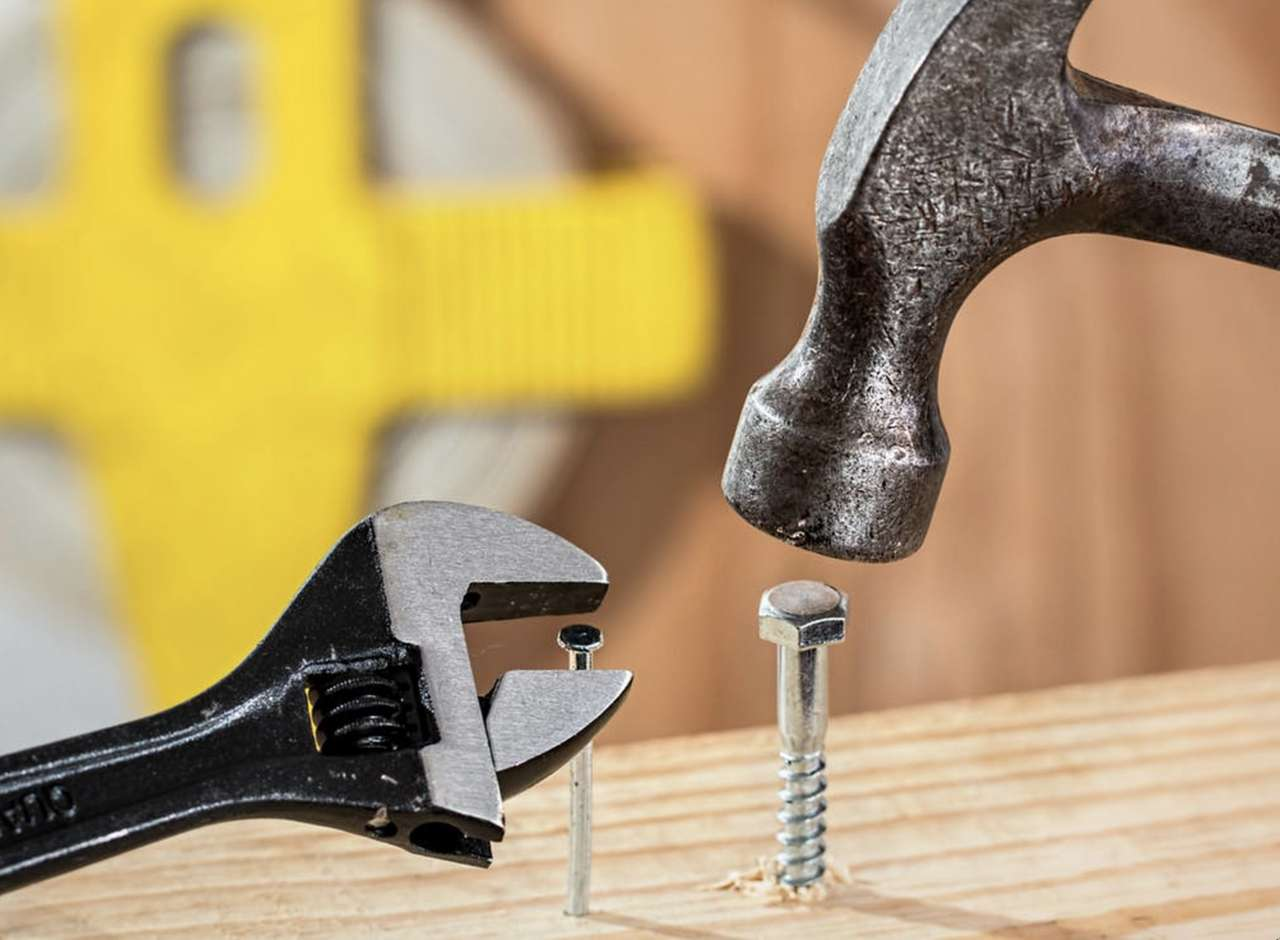
\includegraphics[width=0.7\textwidth]{images/presentacion/tools.jpg}
\end{columns}
\end{frame}

%------------------------------------------------

\begin{frame}{Errores silenciosos y trazabilidad}
\begin{columns}[T]
\column{0.5\textwidth}
\textbf{Riesgo cítico:}

\begin{itemize}
    \item el sistema produce resultados plausibles pero incorrectos.
\end{itemize}
\vspace{1em}
\textbf{Soluciones:}

\begin{itemize}
    \item Logging detallado,
    \item Trazabilidad de evidencias,
    \item Auditoría de decisiones.
\end{itemize}
\vspace{1em}
\textbf{Sin trazabilidad, el sistema no es confiable.}

\column{0.5\textwidth}
\vspace{2em}
\centering

\includegraphics[width=0.8\textwidth]{images/presentacion/amongus.png}
\end{columns}
\end{frame}

%------------------------------------------------

\begin{frame}{Latencia y coste acumulado}
\begin{columns}[T]
\column{0.5\textwidth}
\textbf{Los agentes pueden:}

\begin{itemize}
    \item ejecutar múltiples herramientas,
    \item generar grandes cantidades de tokens,
    \item realizar múltiples iteraciones.
\end{itemize}
\vspace{1em}
\textbf{Resultado:}

\begin{itemize}
    \item latencias elevadas,
    \item costes operativos altos.
\end{itemize}
\vspace{1em}
\textbf{Optimizar flujo es esencial.}

\column{0.5\textwidth}
\centering

\includegraphics[width=0.5\textwidth]{images/presentacion/cost.png}
\end{columns}
\end{frame}

%------------------------------------------------

\begin{frame}{Dependencia de la calidad de los datos}
\begin{columns}[T]
\column{0.5\textwidth}
Si los datos son incorrectos:

\begin{itemize}
    \item el agente amplifica errores,
    \item las conclusiones pueden ser erróneas,
    \item aumenta el riesgo en decisiones deportivas.
\end{itemize}
\vspace{1em}
\textbf{Regla: garbage in → garbage out.}
\column{0.5\textwidth}
\vspace{1em}
\centering

\includegraphics[width=0.6\textwidth]{images/presentacion/calidad.jpg}
\end{columns}
\end{frame}

%------------------------------------------------

\begin{frame}{Principios para agentes robustos}
\begin{columns}[T]
\column{0.5\textwidth}
\begin{itemize}
    \item Validar entradas y salidas.
    \item Limitar iteraciones y costes.
    \item Registrar decisiones y evidencias.
    \item Diseñar flujos controlados por estado.
    \item Mantener supervisión humana.
\end{itemize}

\vspace{1em}
\textbf{Conclusión: robustez > autonomía.}
\column{0.5\textwidth}
\centering

\includegraphics[width=0.6\textwidth]{images/presentacion/gym.jpg}
\end{columns}
\end{frame}



%------------------------------------------------
\section{Conclusiones}
\frame{\sectionpage}

\begin{frame}{Lecciones aprendidas}
\textbf{1. Un agente no es un LLM con más prompts}
\begin{itemize}
    \item Es un sistema que percibe, decide y actúa.
    \item El LLM es el motor de decisión, no el sistema completo.
\end{itemize}

\vspace{0.4em}

\textbf{2. El valor real surge de integrar herramientas y datos}
\begin{itemize}
    \item Los agentes delegan cálculos y consultas a tools externas.
    \item La precisión proviene de combinar IA generativa y procesos deterministas.
\end{itemize}

\vspace{0.4em}

\textbf{3. El control del flujo y del estado determina la robustez}
\begin{itemize}
    \item Arquitecturas dirigidas por estado evitan comportamientos erráticos.
    \item Sin control del flujo aparecen loops, errores y costes excesivos.
\end{itemize}

\vspace{0.4em}

\textbf{4. La memoria y la trazabilidad permiten sistemas fiables}
\begin{itemize}
    \item Registrar evidencias y decisiones es esencial para confiar en el sistema.
\end{itemize}

\vspace{0.6em}

\textbf{Conclusión:} los agentes no añaden “inteligencia mágica”;  
permiten construir sistemas que toman decisiones útiles en entornos reales.
\end{frame}

\end{document}
